%!TEX root = report.tex

\chapter{Experimental Approaches}

This chapter begins by presenting the overall rationale for the experimental
approach used to evaluate the theoretical model.

The primary challenge of analysing the usefulness of the Felemban-Ekici model
lies in the practical problem of accurately capturing network performance
statistics. In total, three different experiments were designed, peformed and
evaluated. Each subsequent experiment lead to a deeper understanding of the
network system and how various systems interact and their effect on the
results.

Any experiment is, by design, constructed and designed in order to observe a
property or behaviour. So that is where this chapter starts -- reasoning about
different parameters of the Felemban-Ekici model. Armed with this set of
parameters, experiment design then becomes a game of exploiting known system
properties and behaviour to obtain a comparable data set.

After selecting intresting properties of the model we then proceed to present
all model evaluation experiments in a chronological order. For each experiment
we try to map the underlying idea to information presented in Chapters 2 and
3. The experiments will relate to an informal and incomplete model of the
system under test and should therefore be read at least twice to answer
questions such as ``if we assume the model to be true, is the experiment
itself sound?'' and ``is the model itself a good enough approximation?''. In
an attempt to spare the reader from inferring incorrect information based on
experiment models, each experiment will be also presented with a short
analysis regarding its soundness.

After describing all model evaluation experiments we continue to present the
experiments designed to test if the stats collected from \texttt{ubus} on the
TG-799 firmware showed any obvious problems.

Finally, we describe a proof-of-concept experiment to evaluate the
Felemban-Ekici model that we ultimately could not perform.


\section{Overview}

As mentioned in the introduction, in order to solve the primary problem as
described in Section 1.3 it has to be partitioned into more manageable pieces.
The problem discussed in this section is ``\emph{Problem 2} - what is a
reasonable definition of \emph{useful}?''.

The premise is as follows: in order to evaluate a theoretical model there must
first exist some set of data provided by the model itself, and an equivalent
set of data to compare against. In this report, the data provided by the model
are referred to as the \emph{model metrics}. The other dataset, the comparison
set, is gathered from a specific device and referred to as the \emph{captured
metrics}.

Since both the original model from Bianchi and Felemban-Ekici models have
strong performance claims backed by evaluations done with simulators the
stated parameters and their behaviour can be considered fact--the models
accurately model IEEE 802.11 performance. What remains unknown is how well
these models perform outside simulations -- on physical hardware using
(imperfect) software drivers. One could argue that since IEEE 802.11 is a
specification all hardware and software that claim to follow that spec. should
be considered equivalent to the spec. and by extension simulators as well.
However, this is in fact an assumption that can serve as a conjecture and
needs to be proven or disproven.

By this reasoning an answer to the original question can be formed:

\begin{itemize}

    \item[\textbf{Q}] \emph{Problem 2} - what is a reasonable definition of \emph{useful}?

    \item[\textbf{A}] Construct an experiment and collect metrics that have
either a direct or indirect equivalent in the theoretical model. If these
metrics match numerically the theoretical model is useful. If these metrics
don't match numerically the theoretical model can still be considered useful
if the trends of these metrics match. If neither of these statments hold, the
model is not useful.

\end{itemize}

The experimental methodology essentially boils down to designing experiments,
based on knowledge of a device and its system, in such a way that the
experiment resulted in a set of \emph{captured metrics} that were comparable
with a predefined set of \emph{model metrics}.

\section{Model Metrics}

As stated earlier, in order to know what to capture we must first select
relevant metrics from the model and the protocol itself. After reading through
\cite{felemban} some variables and parameters are of particular interest:

\begin{itemize}
	\item \emph{N} -- number of network nodes
	\item \emph{D} -- per-packet payload size distribution
  \item $U$ -- normalized throughput (wrt. channel bit rate)
  \item $P$ -- conditional packet collision probability
  \item $T$ -- channel access delay
	\item RTS/CTS -- the model presents models with basic access, RTS/CTS and a
	hybrid access scheme using a payload threshold
\end{itemize}

In addition to these, there are also some parameters and variables that are
used in \cite{felemban} but originate from IEEE 802.11 itself:

\begin{itemize}
    \item channel bit rate
    \item $L$ -- the \texttt{ShortRetryLimit}
    \item $CW_{min}$ and $CW_{max}$ -- contention window min and max size
\end{itemize}


There are, of course, other parameters in the model, and certainly many more
parameters in the implementations of IEEE 802.11 (e.g. power saving, distance,
line-of-sight). These are, for the sake of tractability and real-world
usefulness, ignored and may contribute to significant errors (although such
errors have yet to be discovered in simulations).

As described earlier, the Felemban-Ekici model provides normalized throughput
($U$), channel access delay ($T$) and conditional packet collision probability
($P$).

Normalized throughput ($U$) is constructed upon the conditional packet
collision probability ($P$), payload size distribution ($D$) and a variant of
channel access delay, see Equation \ref{eq:ufe}.

Thus the most important \emph{model metrics} are \emph{conditional packet
collision probability} ($P$) -- the probability that a packet collides during
transmission -- and \emph{channel access delay} ($T$), defined as ``the time
from the packet becoming the head of the queue until the acknowledgment frame
is received.''.

\emph{Conditional packet collision probability} ($P$) is a simple metric,
``count the number of transmission attempts and collisions'', but not an easy
metric to obtain since it occurs at a very low level in the networking stack.
A possible alternative is the \emph{packet drop probability} $P^{L+1}$ -- the
probability of exceeding the short retry limit. The Linux networking system
reliably reports transmission success and failure, but not attempts.

The \emph{channel access delay} ($T$) can be obtained by measuring the total time
described in Figure \ref{fig:timings}. Such a solution would require radio
equipment not available for this thesis. A key insight is that, in a
controlled experiment, most of the parameters in Figure \ref{fig:timings}
are actually constant. The only dynamic parameter is the time spent in
backoff, $T_{\text{BACKOFF}}$.

To summarize,

\begin{itemize}

    \item[\textbf{Q}] \emph{Problem 3} - what data should be collected?

    \item[\textbf{A}] The number of network nodes ($N$), conditional
    packet drop probability $P^{L+1}$, channel access delay ($T$), payload
    size $D$, channel bit rate, retry limit ($L$) and
    contention window sizes $CW_{min}$ and $CW_{max}$.

\end{itemize}

With a set of well-defined \emph{model metrics} we need to collect equivalent
data ponts for, we now move on to describe the experiments, which provide an
answer to ``\emph{Problem 4} - how should this be done?''.

% TODO: flytta till diskussion
% However, after implementing the model, severe differences regarding the
% normalized throughput were discovered. While the re-implementation achieves
% packet collision probabilities similar to the original paper, no realistic
% tuning of throughput calculation parameters could reproduce the original
% values found in the paper. Thus this value is not generated by the
% re-implemented model, but rather compared to the curves found in the paper.

\section{Experiment 1: Wireshark}

% 	\item jana + wireshark pcap time capture (naive) -- A first attempt at
% 	capturing network timing statistics using Wireshark (libpcap).

The first experiment was based on the industry-standard Wireshark program to
capture outgoing packets. Built on libpcap, Wireshark uses a Linux kernel
feature called "packet taps" to "capture" packets. Wireshark records the
packet itself and some related timing data in a log file in a ``pcap'' format.

Naively, the corresponding \emph{channel access delay} was thought to be
obtainable to comparing the timestamps between a send program's call to
\texttt{sendto} and the ``capture time'' reported by Wireshark, as seen in
Figure \ref{fig:wstiming} (experiment timing model, i.e. ``the model which
makes the experiment work''). This would, in fact, be comparable to the
complete timeline from Figure \ref{fig:timings}. No \emph{captured metric}
comparable to \emph{conditional packet collision probability} could be
constructed, simply due to the fact that Wireshark is too high-level to know
about IEEE 802.11 frame transmission failures.

\begin{figure}
\center
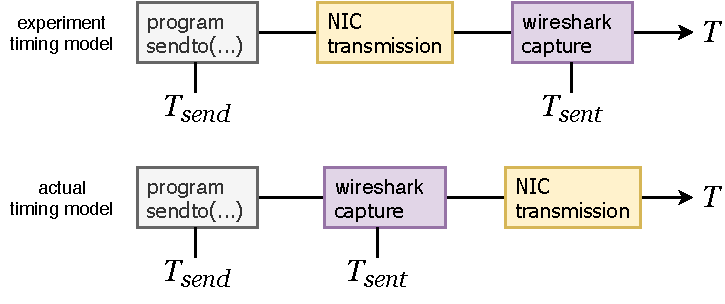
\includegraphics[width=0.7\textwidth]{images/wireshark-experiment-overview.pdf}
\caption{Experiment 1: Wireshark, experiment design vs actual timing models}
\label{fig:wstiming}
\end{figure}

The experiment was designed as follows:

\begin{enumerate}
  \item device \texttt{R}, a TG799-vac router
	\item device \texttt{S}, connected via ethernet to \texttt{R}, running \texttt{jana} in server mode
	\item device \texttt{C}, connected via Wi-Fi to \texttt{R}, running \texttt{jana} in client mode with
  no specified inter-packet latency distribution (a.k.a saturation mode)
	\item wireshark running on \texttt{C}, captures outgoing packets to \texttt{S}
\end{enumerate}

On \texttt{C}, placing the socket in non-blocking mode (\texttt{O\_NONBLOCK}),
\texttt{jana} can detect whenever the socket buffer is full and avoid
measuring the time it took for the kernel to free some memory for the blocked
packet.

With valid values for $T_\text{send}$ and $T_\text{sent}$, we can obtain the
time it took to transmit this packet, or something roughly equivalent to the
\emph{Channel access delay} by taking the difference $T_\text{sent} -
T_\text{send}$

However, the $T_\text{sent}$ timestamp obtained from Wireshark/libpcap is not
what one would expect and for our purposes this divergence between what we
expected and what libpcap delivered was too great to contiune this line of
experimentation. In Chapter 6 we will discuss the underlying reasons for this
in more detail.

\section{Experiment 2: Queueing the Network System} \label{sec:experiment2}

As the Wireshark-based approach seemingly crashed into a hard wall, insights
gleaned from the numerous attempts made to salvage it hinted at a more
theoretical and academic design. \emph{What if we modelled the whole
networking stack as a queueing system? Wouldn't the properties we were looking
for simply be properties of this system?}

The insight that finally ties these loose ideas together, is that a
kernel-owned buffer, known as the \texttt{sndbuf}, owns the memory of each
packet currently being transmitted or received on a particular socket. The
full lifecycle is shown in Figure \ref{fig:linux_egress} and is summarized
here. Some code calls into \texttt{sendto} or \texttt{sendmsg}, which attempts
to allocate memory from the \texttt{sndbuf}, before potentially running tcp,
udp or ip processing filters and finally enqueueing the packet in the qdisc.
The kernel manages pumping packets from the qdisc into the NIC driver. After
transmission, the NIC driver/hardware signals the kernel that packets were
transmitted or dropped. The kernel puts these packets on a ``to free'' list
and eventually frees the related memory, allowing new packets to be allocated
from the \texttt{sndbuf}.


\begin{figure}
\center
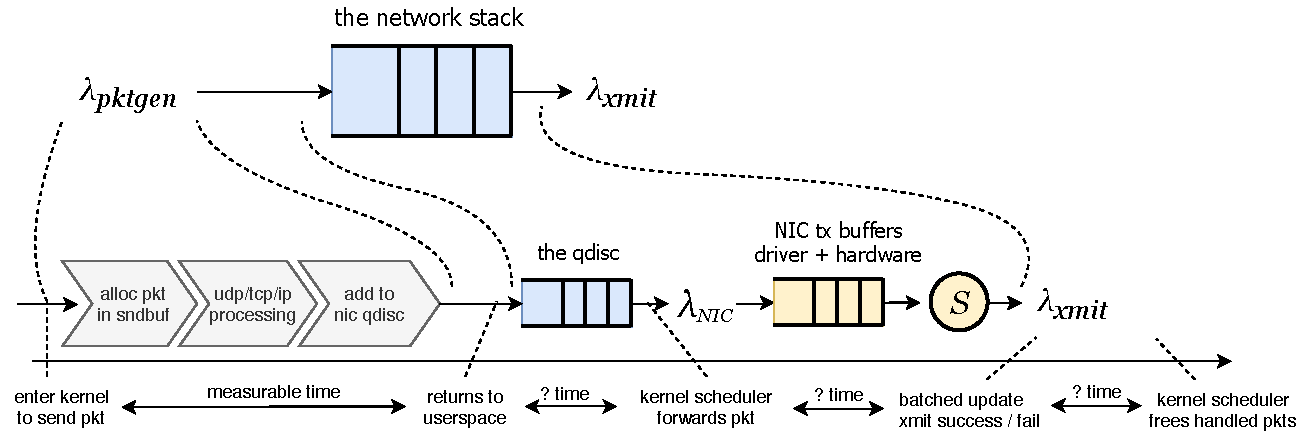
\includegraphics[width=0.9\textwidth]{images/the-network-queue.pdf}
\caption{Experiment 2: Modelling the egress path of a packet as a queueing system}
\label{fig:exp2_overview}
\end{figure}

Modelling the network stack as a M/M/1/K system with K queue length, where K
is

\begin{equation}
K = \frac{\mathtt{sndbuf}}{E[D] + \mathit{kernel~overhead}}
\end{equation}

where $E[D]$ is the average payload size and \emph{kernel overhead} a constant
per-packet bookeeping overhead.

The qdisc queue length is known, and the number of packets currently in the
qdisc system can be queried. Packets can either be owned by the qdisc or the
NIC and so, by assuming that the \texttt{sndbuf} is full, the number of
packets in the NIC queue system can be computed as

\begin{equation}
\label{eq:sndbuf}
L_\text{NIC} = K - L_\text{qdisc}
\end{equation}

We know have an equation for the number of packets in the NIC queue system of
Figure \ref{fig:exp2_overview}. Recall Little's Law, $L = \lambda W$, which,
in this context, states that the average number of packets $L$ in the
networking system is equal to the generation rate multiplied by the average
time $W$ each packet spends in the networking system. This law is applicable
to any arrival process and service distribution, and crucially, it's also
applicable to any subsystems as well.

With Little's Law we can obtain the service time $W_\text{NIC}$ of a packet,
i.e the average time a packet spends at the server. The exact definition of
$W_\text{NIC}$, assuming a stable flow of packets and mostly full
\texttt{sndbuf}, becomes

% \begin{equation}
\begin{align}
\label{eq:wnic1}
    L_\text{NIC} &= \lambda_\text{NIC} W_\text{NIC}         && \text{Little's Law}\nonumber\\
    W_\text{NIC} &= \frac{L_\text{NIC}}{\lambda_\text{NIC}} && \text{isolate service time}~W_\text{NIC}\nonumber\\
    W_\text{NIC} &= \frac{K - L_\text{qdisc}}{\lambda_\text{NIC}} && \text{substitute}~L_\text{NIC}~\text{from Equation \ref{eq:sndbuf}}
\end{align}
% \end{equation}

Furthermore, $W_\text{NIC}$ can be deconstructed as shown in Figure
\ref{fig:timings} plus a term for time spent waiting in the queue, and
provides the final link how $W_\text{NIC}$ relates to the variable we are
looking for, $T_\text{BACKOFF}$

\begin{align}
\label{eq:wnic}
W_\text{NIC} =&~T_\text{QUEUE} + T_\text{DIFS} + T_\text{BACKOFF} \nonumber\\
              &+ T_\text{PHY} + T_\text{MAC} + T_\text{FRAME}\\
              &+ T_\text{SIFS} + T_\text{ACK}\nonumber
\end{align}

%todo :add these to background IEEE section Recall that \texttt{SIFS} and
Where $T_\text{QUEUE}$ is the time spent waiting to be served, $T_\text{DIFS}$
and $T_\text{SIFS}$ are the interframe spaces defined in IEEE 802.11 and set
by the access point \cite{654749}, $T_\text{PHY}$ the preamble, $T_\text{MAC}$
time to send MAC header and $T_\text{ACK}$ the time for a special \texttt{MAC}
packet. Simply, \texttt{DIFS} and \texttt{SIFS} depend on network
configuration whereas \texttt{PHY}, \texttt{MAC}, \texttt{FRAME} and
\texttt{ACK} primarily depend on channel bit rate, guard interval and time
quantization ($T_\texttt{slot}$).

Some practical problems had to be resolved:

\begin{enumerate}

  \item Fast polling of the qdisc queue, solved by hacking the \texttt{tc}
(traffic control) program, see
\url{https://github.com/smeets/thesis/tree/master/d3fi/tcq}

  \item A full qdisc will sliently drop new packets, solved by increasing the
  max queue length using \texttt{ifconfig txqueuelen}

  \item The NIC should at all times be maxed out, solved by increasing the
\texttt{sndbuf} size by increasing kernel parameters
\texttt{/proc/sys/net/core/wmem\_max} (UDP \texttt{sndbuf} maximum size) and
\texttt{/proc/sys/net/core/wmem\_default} (UDP \texttt{sndbuf} default size)
to 10 MB. Combined with a large qdisc size this should allow the kernel to
always have packets to pump into the NIC.

\end{enumerate}

The complete experiment:

\begin{enumerate}

  \item Start a UDP-spam process, see
  \url{https://github.com/smeets/thesis/tree/master/d3fi/ethx.py}

  \item Get the active inode from \texttt{/proc/net/udp}

  \item Log data from the specified iface and inode, see
  \url{https://github.com/smeets/thesis/tree/master/d3fi/data1.sh}, using data
  from \texttt{tcq}, \texttt{ethtool} and \texttt{procfs} device \texttt{/proc/net/udp}

  \item Send log data into a web server,
  \url{https://github.com/smeets/thesis/tree/master/d3fi/server.js}, which
  stores the data and makes it available to a browser

  \item A browser on the local host that loads a page from above server and
  periodically fetches new log data

\end{enumerate}

The primary issue with this approach is related to how the kernel keeps
already transmitted packets for an unknown amount of time before freeing the
packet data in batches, increasing overall system throughput.


\section{Experiment 3: Hacking on the driver}

Compared to the previous attempt, a more practical approach would be to try
and observe whenever packets are handed over to the NIC from qdisc and handed
over from the NIC back to the kernel. Sampling this process would then give an
estimate for the number of packets enqueued in the NIC.

This is in fact how the third and final experiment started: \emph{``Where in
the kernel can we log qdisc $\rightarrow$ NIC and NIC $\rightarrow$ kernel
handover events?''}. The anwer, of course, is \emph{``in the NIC driver''}.

While exploring in-tree wireless drivers a suspicious field appeared in a
driver for intel wireless NICs (\texttt{iwlwifi}),
\texttt{wireless\_media\_time}, described as

% \begin{lstlisting}[language=c++,caption={snippet from tx.h},label=lst:iwlwifi]
% /* @wireless_media_time:
%  *  for non-agg: RTS + CTS + frame tx attempts time + ACK.
%  *  for agg: RTS + CTS + aggregation tx time + block-ack time.
%  *  in usec.
% \end{lstlisting}


\begin{verbatim}
* @wireless_media_time:
 *  for non-agg: RTS + CTS + frame tx attempts time + ACK.
 *  for agg: RTS + CTS + aggregation tx time + block-ack time.
 *  in usec.
\end{verbatim}

and while this description appears to include some components from Figure
\ref{fig:timings}, the comment is too vague to form any definition. Some
notes:

\begin{itemize}

\item ``wireless media time'' should, in our opinion, refer to the total
duration the wireless medium was used. This implies that backoff is not
included and that frame transmission time is included. However, the comment
indicates the opposite.

\item Consumer Wi-Fi networks often use a hybrid access mode, defaulting to
basic and only sending RTS/CTS frames if the payload size exceeds some
threshold. In our case this threshold is greater than the maximum amount of
payload a IEEE 802.11 frame can contain, which implies that RTS/CTS will never
be used in our setup.

\item ``frame tx attempts time'' could include any combination of BACKOFF, PHY,
MAC and FRAME components. It is possible to probe some of these components,
e.g. varying payload size should give a corresponding impact if FRAME is
included, BACKOFF can be proved by changing number of STAs.

\end{itemize}

In any case, the primary objective is to observe if this field is of use.
Figuring out exactly what ``frame tx attempts time'' is tricky. We can,
however, run multiple experiments with varying payload sizes and active
network clients to see if backoff or time spent transmitting data are
included.


\begin{figure}
\center
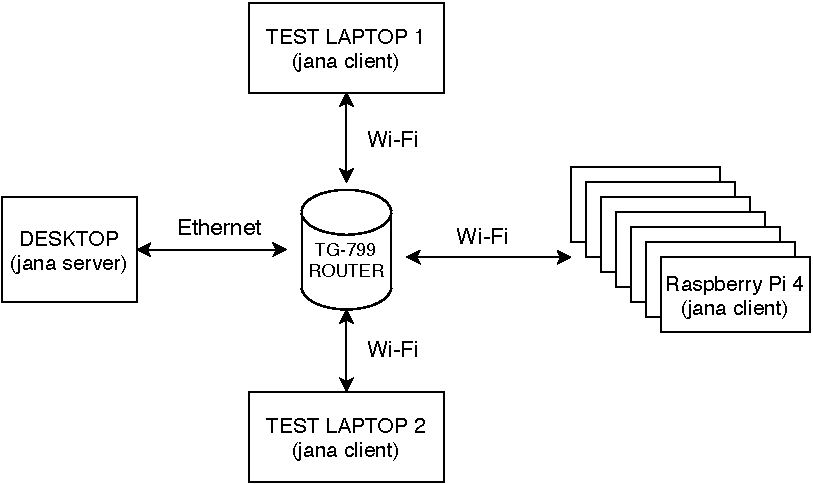
\includegraphics[width=0.9\textwidth]{images/exp3-overview.pdf}
\caption{Experiment 3: Hacking the Wi-Fi driver setup overview}
\label{fig:exp3_overview}
\end{figure}


Our testbed, as shown in Figure \ref{fig:exp3_overview}, consists of

\begin{enumerate}
  \item a TG-799 router
  \item one desktop, running the jana server (connected via ethernet)
  \item 20 Raspberry Pi 4, acting as network load generators (connected via Wi-Fi)
  \item one laptop with modified Wi-Fi driver (connected via Wi-Fi)
  \item one control laptop with modified Wi-Fi driver (connected via Wi-Fi)
\end{enumerate}

The two laptops used the modified Wi-Fi driver to log the
\texttt{wireless\_media\_time} throughout the test. Both laptops ran the jana
client, sending UDP packets to the server running on the desktop, which was
connected via ethernet. An ethernet connection was chosen since Wi-Fi uses a
shared medium, which means that communication is simplex. By connecting the
server via ethernet, we can assume that the cost of forwarding packets from
Wi-Fi to Ethernet is so low that it can be ignored for our experiments. In
addition to the two laptops we set up a number Raspberry Pi 4s to also run the
jana client and send UDP packets to the jana server, with the intention
increase the load on the CSMA algorithm and risk of Wi-Fi frame collisions,
which in turn affects the backoff process.

The experiment was parameterized on payload size and number of active jana
clients. Packet generation distribution was fixed to ``as many as possible''.

The hypothesis is that varying payload size would reveal if
\texttt{wireless\_media\_time} contained any transmission timings, and varying
the number of active jana clients (i.e varying medium contention) would reveal
any backoff timings.

The number of clients were ${5,10,15,20}$ and payload sizes varied from 1 byte
to 32 kilobytes (1, 2, 4, 8, ...). Note that the maximum IEEE 802.11 frame
size is around 1460 bytes, so any packet jana generates with a payload larger
than approximately 1KB will result in multiple IEEE 802.11 frames being
transmitted. Intuitively, the per-frame wireless media time should remain
constant while the per-packet latency should increase linearly with the number
of frames requires to fully transmit the packet.



\section{Evaluating: In the Wild}

Evaluating the model under controlled conditions (``in the lab'') is only one
part of the analysis. How the model performs ``in the wild'' is a natural next
step and in this section we will describe the methodology behind our model
evaluation, ``in the wild''.

Since we cannot expect end-users to load logging programs we must either run a
logger on a network client or log directly from the router. We do not have
access to a programmable radio so we will attempt to acquire metrics directly
from the router.

The network interface metrics can be accessed through various different
interfaces. In this thesis two programs were tried during exploratory testing,
\texttt{ubus} and \texttt{quantenna api}. In the end \texttt{ubus} was chosen
due to its broader range of statistics (both 2.4 and 5 GHz modems, compared to
only 5 GHz for quantenna) and consistency of its output (no corrupt/invalid
JSON was detected, compared to some corrupted output for quantenna). Since
both interfaces report metrics from the same sources (from kernel, driver and
firmware) we should get roughly equivalent data points no matter the
interface.

In conclusion, network performance metrics will be collected by periodically
calling the \texttt{ubus} program on the router.

\subsection{Selecting ubus metrics}

After deciding \emph{how} to collect data, it is time to decide \emph{what}
data to collect.

As mentioned earlier, the model parameters form our comparison set. Data
collected during testing needs to map directly or indirectly to the comparison
set. It makes sense, then, to start with model parameters and try to find
equivalent metrics.

\begin{itemize}

    \item \emph{network nodes (N)} - maps directly to number of connected network clients. We exclude
    the router from this number as it will never attempt to transmit volountarily.

    \item \emph{channel bit rate} - the bit rate used to transmit and receive.
    Expressed in physical tx/rx rates in most drivers and indicated by the
    Modulation and Coding Scheme (MCS) index. It is important to note that even if
    IEEE 802.11 n can transmit up to 600 Mbps, the advertised bit rate will depend
    on signal strength, number of MIMO antennas, guard interval, bandwidth and
    other factors. Therefore, it is better to log the physical tx/rx rates
    actually used instead of using the theoretical maximum.

    \item \emph{normalized throughput (U)} - is estimated in the model as average time
    spent transmitting payload vs. total system time. This is roughly equal to the average
    throughput of the system divded by the advertised channel bit rate. Average network throughput
    can be obtained by computing $ 8 \frac{ \text{RX}_\text{ bytes } }{ \text{time} } $ (from router's point of view).

    \item \emph{packet collision probability (P)} - refers to the IEEE 802.11
    frame collision probability and as far as we researched, must be obtained from
    the NIC. Our NIC does not provide this information. An alternative is to count
    the number of dropped packets, i.e. packets dropped by the NIC due to
    exceeding the maximum number of retransmission attempts. The model defines
    this property as $P^{L+1}$, where $P$ is the conditional collision probability
    and $L$ the retry limit.

\end{itemize}

In addition to these metrics, we decided to include the Received Signal
Strength Indicator (RSSI), a vendor-specific metric which can be used to gauge
signal strength, in case our experiments showed any unexpected behaviour.

\subsection{Analysing ubus metrics}

As good scientists we should not take data at face value. Thus we decided to
conduct some experiments to sanity check the reported metrics. For each
selected metric a test was performed to try and uncover any unexpected
behavior.

\begin{itemize}

    \item \emph{network nodes (N)} - read directly from \texttt{ubus} output

    \item \emph{channel bit rate} - physical rx/tx rates read directly from \texttt{ubus}

    \item \emph{normalized throughput (U)} - the $\texttt{RX}_\texttt{bytes}$ was read directly from \texttt{ubus}

    \item \emph{packet collision probability (P)} - dropped backets read directly from \texttt{iwconfig}

\end{itemize}

The test: log periodically on a router running iperf3 in server mode with one client
running iperf3 in client mode during 12 hours.


\subsection{RSSI experiments}

Received Signal Strength Indicator (RSSI) is an important, and tricky, value. It
is important because it is often the only indicator of signal strength, and
tricky due to high variance between two chips, from same or different vendors,
suggesting that variance stems from a combination of hardware and software
factors \cite{lui}.

In order to establish whether the RSSI metric could be used or not, analysis had
to be done to verify the behavior, accuracy and variance of the reported values.
This was done in a shielded lab with low-to-no external interference and no self
interference from reflection.

Figure \ref{fig:rssi_setup} shows how the router, antenna and laptop were
set-up. Three experiment sessions were carried out to measure RSSI, about 5
minutes per session, with two different spectrum analysers.

The first test established the baseline rssi values when the system (laptop) was
idle, i.e. any network load originated from background services. The second test
was conducted using \texttt{iperf3} to push as much network load as possible,
see listings \ref{lst:router}, \ref{lst:client} and \ref{lst:rssi} for relevant
scripts. The third test was a control test with a different spectrum analyser,
but otherwise identical to the second test.

Scripts for parsing the spectrum analyser data and related heat map generator
are detailed in listings \ref{lst:mdrparse} and \ref{lst:mdrplot}.

The \emph{spectrum analyser data} was plotted as a heat map; frequency vs. time
vs. signal strength. This graph shows both how signal strength varies over time
and frequency. In contrast, the \emph{router metrics} only specify one RSSI
value and thus the resulting plot compares RSSI vs. time. The graphs can be
analysed individually for insight into system behavior and compared to see how
they relate.

We did not have time to get the second spectrum analyser to output data as a
fuse went during our first attempt with it and we had to wait for it to be
fixed. On the other hand, this spectrum analyser was used to calibrate and
estimate the attenuation of the antenna cable. In the end this analyser was
mainly used to eyeball that the first spectrum analyser was somewhat correct
and to estimate cable attenuation.

\begin{figure}
\center
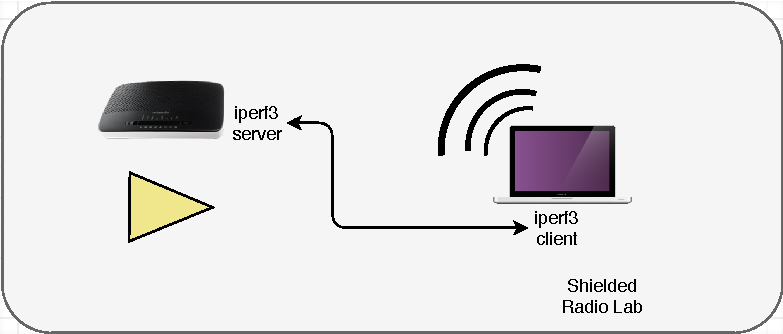
\includegraphics[width=0.9\textwidth]{images/rssi-exp.pdf}
\caption{TG799 router and measurement antenna side by side, 1 meter from laptop}
\label{fig:rssi_setup}
\end{figure}

\subsection{Evaluation}

Armed with a solid set of \emph{router metrics} data collection could begin.

To compare our collected data against the model we first implemented the model
as a program, see Listing \ref{lst:efmodel} in the Appendix. As a preliminary
test of the implementation we tried to compare our model with the numbers
published in \cite{felemban}, and were surprised that only the
\emph{conditional collision probability} was correct: neither \emph{normalized
throughput} nor \emph{channel access delay} were correct. Since this could be
caused by different parametrisation we attempted to find possible parameters
using a brute-force approach, but this resulted in skewed and unsound
parameters. So we reached out to the authors of the model in order to try and
obtain the original source code. After a week we got a reply that it could
take a while to dig stuff that old up and waited, but nothing arrived and we
received no response to subsequent email attempts.

Thus it became impossible for us to evaluate the model.
